\documentclass[12pt]{article}
%\usepackage{fullpage}
\usepackage{epic}
\usepackage{eepic}
\usepackage{paralist}
\usepackage{graphicx}
\usepackage{tikz}
\usepackage{xcolor,colortbl}

\usepackage{fullpage}
\usepackage{amsmath,amsthm,amssymb}
\usepackage{algorithmicx, algorithm}
\usepackage[noend]{algpseudocode}

\newcommand*\Let[2]{\State #1 $\gets$ #2}
\newtheorem{theorem}{Theorem}
\newtheorem{lemma}[theorem]{Lemma}
\newtheorem{proposition}[theorem]{Proposition}
\newtheorem{corollary}[theorem]{Corollary}

\newenvironment{definition}[1][Definition]{\begin{trivlist}
\item[\hskip \labelsep {\bfseries #1}]}{\end{trivlist}}
\newenvironment{example}[1][Example]{\begin{trivlist}
\item[\hskip \labelsep {\bfseries #1}]}{\end{trivlist}}
\newenvironment{remark}[1][Remark]{\begin{trivlist}
\item[\hskip \labelsep {\bfseries #1}]}{\end{trivlist}}

\newcommand*\Th[1]{{#1}^{\textrm{th}}}

%%%%%%%%%%%%%%%%%%%%%%%%%%%%%%%%%%%%%%%%%%%%%%%%%%%%%%%%%%%%%%%%
% This is FULLPAGE.STY by H.Partl, Version 2 as of 15 Dec 1988.
% Document Style Option to fill the paper just like Plain TeX.

\typeout{Style Option FULLPAGE Version 2 as of 15 Dec 1988}

\topmargin 0pt
\advance \topmargin by -\headheight
\advance \topmargin by -\headsep

\textheight 8.9in

\oddsidemargin 0pt
\evensidemargin \oddsidemargin
\marginparwidth 0.5in

\textwidth 6.5in
%%%%%%%%%%%%%%%%%%%%%%%%%%%%%%%%%%%%%%%%%%%%%%%%%%%%%%%%%%%%%%%%

\pagestyle{empty}
\setlength{\oddsidemargin}{0in}
\setlength{\topmargin}{-0.8in}
\setlength{\textwidth}{6.8in}
\setlength{\textheight}{9.5in}


\setcounter{secnumdepth}{0}


\setlength{\parindent}{0in}
\addtolength{\parskip}{0.2cm}
\setlength{\fboxrule}{.5mm}\setlength{\fboxsep}{1.2mm}
\newlength{\boxlength}\setlength{\boxlength}{\textwidth}
\addtolength{\boxlength}{-4mm}

\newcommand{\algobox}[2]{
  \begin{center}
    \framebox{\parbox{\boxlength}{
        \textbf{Introduction to Algorithms} \hfill \textbf{#1}\\
        \textbf{CS 4820, Spring 2014} \hfill \textbf{#2}}}
  \end{center}}

\newcommand{\algosolutionbox}[2]{
  \begin{center}
    \framebox{\parbox{\boxlength}{
        \textbf{CS 4820, Spring 2014} \hfill \textbf{#1}\\
        #2
      }}
  \end{center}}


\begin{document}

\algosolutionbox{Homework 5, Problem 1}{
  % TODO: fill in your own name, netID, and collaborators
  Name: Piyush Maheshwari\\
  NetID: pm489\\
  Collaborators: Eeshan Wagh
}

\bigskip

\textbf{(1)}
\emph{(10 points)}

Consider the following generalization of the median-finding problem:
given a sequence $A=(a_1,\ldots,a_n)$ and integers $k_1< k_2 < \dots <k_t$ between $1$ and $n$,
output a sequence $B=(b_1,\ldots,b_t)$ such that $b_i$ is the $(k_i)^{\mathrm{th}}$ largest element among the elements in $A$ for all $i$ from $1$ to $t$.
You may assume the elements of $A$ are all distinct.

Show that there exists a randomized algorithm for this problem with expected running time $O(n\log t)$.

Since a sorting-based algorithm can solve this problem in time $O(n\log n)$, 
the interesting case for the algorithm occurs when $\log t$ is significantly 
smaller than $\log n$. Accordingly, algorithms that solve the problem by 
sorting the entire sequence $(a_1,\ldots,a_n)$ will not be considered
acceptable solutions to this problem.

 \bigskip

\subsection{Solution}

We will use select(k,S) algorithm covered in class as a subroutine to this problem. Initially we have n elements in A and t values of $k_i$.

The algorithm will be recursive. In each call to the algorithm, we will pick the mid point of the array of numbers from ($ k_1.... k_t$) = $k_{t/2}$ and then call select(n,$k_{t/2}$) to find the $k_{t/2}$ largest element in the array from $(a_1,...a_n)$. Suppose that element is $a_x$. Store this element in $b_{t/2}$. Now if we split the array into two arrays $A_l$ and $A_r$ such that all elements in $A_l$ are smaller than $a_x$ and all elements in $A_r$ are greater then $a_x$. Since all the k's are in increasing order, we know that all $k_i$'s before $k_{n/2}$ will be in $A_l$ and all $k_i$'s after $k_{n/2}$ will be in $A_r$. Hence we can recursively solve these smaller sub problems. We will stop our recurrence when there is only a single value of k passed in the recursive method. In that case we will simple call select(k,S) and output the answer.

\subsection{Proof of Correctness}

We can prove the correctness by induction. 
We claim that find-median(n,t) correctly outputs the sequence $(b_1, b_2,..b_n)$.


\underline{Base case}

Consider find-median(n,1). In this method we  have only one value of k. Since in this we will only call select(n,k), this will out the correct answer assuming the correctness of select(n,k).

\underline{Inductive Step}

Consider find-median(n,t). We find the mid point among the 't' values of k's and call select(n,$k_{t/2}$). Then we partition the array A into two arrays $A_{l}$ (some size x) and $A_{r}$(size n-x-1) and recursively call find-median(x, (t-1)/2) and find-median(n-x-1, (t-1)/2). Using inductive hypothesis we claim both these recursive calls will correctly compute the array b[]. Using this fact and the fact that select(n,$k_{t/2}$) will correctly compute the largest t/2 element, we will get all the value of $b_i$. Thus the induction holds.

\subsection{Running Time}

Assume the size of $A_l$ that we compute in any recursive call is x. Then the size of $A_r$ is n - x - 1. From lecture we know that select (n,k) takes O(n) time. \\\\
The recurrence can be represented as T(n,t) = T(x,t/2) + T(n-x-1, t/2) + O(n)
\\\\
If we draw the recursion tree of this recurrence, we can easily see that there is at each level of tree, we do O(n) work. This is because the sum of subproblems that we have at any stage is O(n).

\begin{tikzpicture}[scale=0.2]
\tikzstyle{every node}+=[inner sep=0pt]
\draw [black] (34.6,-12.5) circle (3);
\draw (34.6,-12.5) node {$O(n)$};
\draw [black] (26.9,-21.2) circle (3);
\draw (26.9,-21.2) node {$O(x)$};
\draw [black] (43.9,-20.5) circle (3);
\draw (43.9,-20.5) node {$O(n-x)$}; 
\draw [black] (18.2,-31.5) circle (3);
\draw (18.2,-31.5) node {$O(y)$};
\draw [black] (30.1,-31.5) circle (3);
\draw (30.1,-31.5) node {$O(x-y)$};
\draw [black] (41.8,-31) circle (3);
\draw (41.8,-31) node {$O(n-x-q)$};
\draw [black] (50.9,-31.2) circle (3);
\draw (50.9,-31.2) node {$O(q)$};
\draw [black] (32.61,-14.75) -- (28.89,-18.95);
\fill [black] (28.89,-18.95) -- (29.79,-18.69) -- (29.04,-18.02);
\draw [black] (36.9,-14.8) -- (41.57,-18.61);
\fill [black] (41.57,-18.61) -- (41.27,-17.71) -- (40.64,-18.49);
\draw [black] (24.96,-23.49) -- (20.14,-29.21);
\fill [black] (20.14,-29.21) -- (21.03,-28.92) -- (20.27,-28.27);
\draw [black] (28.1,-24) -- (29.33,-28.6);
\fill [black] (29.33,-28.6) -- (29.6,-27.7) -- (28.64,-27.96);
\draw [black] (43.31,-23.44) -- (42.39,-28.06);
\fill [black] (42.39,-28.06) -- (43.04,-27.37) -- (42.05,-27.18);
\draw [black] (45.8,-22.9) -- (49.33,-28.64);
\fill [black] (49.33,-28.64) -- (49.34,-27.7) -- (48.48,-28.22);
\end{tikzpicture}and so on.
\\\\
We can easily see that the amount of work done on each level is O(n). And since we are dividing the value of t by half at each level, the depth of the tree with be log(t). \\\\
Hence the total running time of the algorithm will be O(n logt)
\end{document}
